\documentclass[a4paper,man,natbib]{apa6}


\usepackage[english]{babel}
\usepackage[utf8x]{inputenc}
\usepackage{amsmath}
\usepackage{float}
\restylefloat{figure}
\usepackage{graphicx}
%\usepackage[section]{placeins}

\usepackage[colorinlistoftodos]{todonotes}
%Unsupervised ranking of person name entities based on reputation.
\title{A Reputation System for Person Name Entities Using Unsupervised Ranking}
\shorttitle{Reputation System}
\author{Haimonti Dutta$^{1}$, Aayushee Gupta$^{2}$, Jayashree Chandrasekharan$^{3}$}
\affiliation{$^{1}$Department of Management Science and Systems, \\
University at Buffalo, Buffalo, NY, 14221. \\
$^{2}$Department of Computer Science, IIIT Bangalore, Karnataka, India. \\
$^{3}$Department of Computer Science, University at Buffalo, Buffalo, NY, 14221. \\
Email: \{haimonti,jchandra\}@buffalo.edu; aayushee1230@iiitd.ac.in}


\abstract{Text databases containing newspaper articles, reports, logs, proceedings, and books have grown tremendously in number, size and volume over the last few decades. They are often stored using large-scale infrastructure (such as parallel and distributed repositories, data clouds) and web interfaces allow access to individual documents in the repository. However, methods for automatic content extraction from text and using them to understand the collections are still lacking in number and scope. In this paper, we address one such problem, namely the task of finding \emph{reputed} people from text repositories. Our goal is to automatically populate a list of person name entities sorted by reputation. For our purposes, a person's reputation depends on several factors including the number of times s/he has been discussed in the text, in what context and relevant details from the narrative.We first design a \textit{gazetteer} to keep track of people names using named entity recognition and coreference resolution of text documents. This is followed by extraction of features to characterize reputation and ranking them using a novel unsupervised rank aggregation scheme. The top-K entries of the ranked lists are evaluated manually by human annotators to assess the relevance of the findings. %The ranked list(s) generated from this study are incorporated into timelines representing important events in a country's history.
Empirical results are presented using two newspaper corpora one comprising of 14020 articles from a historical newspaper, ``The Sun", published from New York in 1896 and another contemporary newspaper ``The Washington Post".}

\begin{document}
\maketitle
\setcounter{secnumdepth}{4}
%\chapter{Introduction}
\section{Introduction}
\label{sec:introduction}
Large scale text repositories storing books, newspaper articles, reports and proceedings have now been in existence for many decades. 
%Historical newspaper archives, for example, have typically grown incrementally first by digitizing a small number of newspapers relevant to a regions history, geographic coverage, and events of a particular time period and subsequently digitizing more papers in phased development. 
They are capable of providing a wealth of information to scholars. The keyword-based retrieval systems designed for these repositories allow access to individual documents, but may often exhibit poor retrieval performance for a variety of reasons such as noisy and garbled\footnote{Optical Character Recognition (OCR) technology used for digitization is imperfect and generates a lot of garbled text.} text, incongruity in language and choice of keywords. The problems with the retrieval systems often contribute to a lack of understanding of the corpora as a whole and may even hinder development of systems for automatic content extraction. 
%Digitization of old newspapers helps to develop a searchable database of newspaper articles which greatly enhances accessibility of such information \cite{yang2011topic}.
%%They
%are of particular interest to genealogists, historians and scholars for \textit{people search} -- the process of finding information about a person and reconnecting them with others they are likely to know. The goal is often to determine who knows whom and how.

This paper addresses one such problem -- that of extraction of names of \emph{reputed} people from text corpora by examining the context in which person names occur, the number of times they appear in the documents and with what frequency, and other features from the text. Such an exercise can help to learn about influential people in the context of a country's timeline of events. They can also aid the process of people search \cite{BilenkoMCRF03,Friedman_92} by finding information about a person. 

While the problem of reputed person detection has been studied extensively in the field of social networks and marketing, our problem is different due to the following characteristics:
\begin{enumerate}
\item Text repositories are not hyperlinked and lack explicit citation structure; this makes the problem at hand fundamentally different from finding influence in citation graphs. 
\item The notion of \emph{reputation} of a person name entity has to be operationalized based on the content and structure of the documents.
\item  The automatically generated ranked lists of reputed people have to be evaluated by human annotators since ground truth is unavailable for the task.  
\end{enumerate}

The premise of this research is that it is possible to extract person name entities from text repositories; each individual reference to the entity must be identified in the corpus and linked together. Entity profiles are then created which contain information pertaining to statistical properties of documents in which the name occurs. This provides a mechanism to rank them using rank aggregation techniques and evaluate the results manually by experts. Following this premise, a \emph{people gazetteer} is generated from noisy OCR text. This organized dictionary of people names is extracted using named entity recognition and coreference resolution of spell corrected text. Following this, entity profiles are generated based on the number of times s/he has been discussed in news, in what topics and other relevant details from the narrative.These profiles are ranked to determine the reputation of these entities. 

%For all of the above use cases, the primary goal is automatic extraction of , since newspapers are scanned by the use of Optical Character Recognition (OCR) technology and this generates a lot of garbled text. Furthermore, particular entity across a set of documents. 



%The goal is to determine who knows whom and how. This may be achieved by studying biography. However, biographies may be largely untraceable for historical groups. In such cases, secondary information (personal testimonies, newspaper articles, etc.) is studied. This process is called \textit{prosopography}
%%Identification of this group of individuals and studying stories of their lives is an important tool in \textit{prosopography}. 
%%In such cases, the common characteristics of a historical group may be learnt by analyses of statistically relevant quantities of biographical data about a well-defined group of individuals.  
%and can be used to learn about social structure, professional and occupational groups or economic classes. %
%Quoting prosopographer Katharine Keats-Rohan, 
%\begin{quote}
%...prosopography is about what the analysis of the sum of data about many individuals can tell us about the different types of connection between them, and hence about how they operated within and upon the institutions -- social, political, legal, economic, intellectual -- of their time.
%\end{quote}

% The nature of prosopographical research has evolved over time. Lawrence Stone\cite{stone_71} discusses an ``older" form of prosopography which was principally concerned with well-known social elites, many of whom were influential people. Their genealogies were well-researched, and social webs and kinship linking could be traced, allowing a prosopography of a ``power elite" to emerge. This older prosopography can be contrasted with a newer form called \emph{quantitative prosopography}, which studied much wider populations including ``ordinary people". %The people gazetteer discussed in this paper primarily deals with quantitative prosopography.

%\noindent In this paper, we present a framework to find reputed people from noisy OCR text. develop a \textit{people gazetteer} which forms the basis of prosopographical research. The gazetteer is built from the text of historical newspapers subjected to Optical Character Recognition (OCR) and is capable of identifying reputed people. Our paper has the following novel contributions: (1) \textbf{Development of the People Gazetteer} -- an organized dictionary of people names is extracted using Named Entity Recognition and Coreference Resolution. (2) \textbf{Ranking of Person Name Entities}: we study two rank aggregation schemes -- Borda and median-based rank aggregation to obtain ranked lists of person name entities. 
%
%To the best of our knowledge, the development of such a framework for doing prosopographical research using machine learning has not been studied before. This exercise, however, opens up a wide range of possibilities -- for example, 
%%news articles related to the influential person can also be linked to a Wikipedia page entry to find out relevant details or 
%to build influential people networks that can learn about entities involved in historical events. Such applications can immensely help historians working on prosopography\cite{allen2013toward} and scholars in learning events related to historically significant people interactively.

\noindent \textbf{Paper Organization:} This paper is organized as follows: Section~\ref{repsys} presents the definition, prior work and design principles for building reputation systems; the reputation system for person name entities is discussed in Section~\ref{pnRep}; empirical results on two datasets -- a historical newspaper archive and Washington Post data are presented in Section~\ref{emp};  Section~\ref{related} discusses related work; and Section~\ref{conc} concludes the paper.

\section{Reputation Systems: Definition, Prior Work and Design Principles}
\label{repsys}

\noindent The Oxford American dictionary defines reputation as beliefs or opinions held about individuals, organizations or things. Often, reputation is role fulfillment (\cite{Carter_02}). It is ascribed by society to an individual and is deemed personal. The opinion held by society about the individual is based on the way his/her identity has been managed and presented to society. Mathematically, reputation is defined as a personalized function of claims, transactions and opinions (\cite{Windley_07a}) i.e.
\begin{equation}
R_p = f(C_p, T_p, O_p)
\end{equation}
where $R_p$ indicates the reputation of a person, $C_p$ is the vector of claims about person $p$, $T_p$ is the vector of transactions and $O_p$ is the associated opinions about $p$. In general, claims are facts about a person that can be verified, opinions are indirect information from other sources while transactions are records of interactions between entities.
Positive reputation is associated with increase in confidence, trust, social status and power. People with positive reputation are sought out by society -- therefore, it is often imperative that a person will try to maximize his/her positive reputation through identity management.

Computational models of reputation (often called reputation systems in literature) are fairly recent (\cite{Sabater_05,Resnick_02}). Resnick et al. (\cite{Resnick_02}) define a reputation system as a system that ``collects, distributes, and aggregates feedback about participants' past behavior". They have been studied in various disciplines including philosophy (\cite{Hume_75}), sociology (\cite{Wasserman_94}), economics (\cite{Milgrom_82}), computer science (\cite{Kamvar_03a}), marketing and social networks (\cite{Dellarocas_03}). They can be analyzed from different perspectives and can be used in a wide range of situations. This often makes them hard to classify. Sabater and Sierra  (\cite{Sabater_05}) provide a conceptual model of reference for reputation systems according to which, reputation systems can be broadly classified into (a) Cognitive models, in which reputation is made up of underlying beliefs and is assumed to be a function of those beliefs and (b) Game theoretic models, in which subjective probabilities are used to characterize the expectation of an individual $A$ who depends on individual $B$ to perform an action on which $A$'s welfare depends. We claim that our system to identify reputed people from large text corpuses is a cognitive model as the reputation of a person is inherently linked to the beliefs that other people have about him/her in the pre-specified time interval. 

\noindent \textbf{Prior Work: } Many online marketplaces including eBay (\cite{eBay_02}), Amazon Auctions (\cite{AA}) and OnSale Exchange (\cite{OnSale}) use reputation systems extensively. For example, items on eBay are sold by English auctions and users provide ratings (positive, negative or neutral) of sellers -- these ratings collected over a pre-determined time frame, are used to design reputation systems. Google's  search results (\cite{Brin_98a}) are ranked by how many sites contain links that point to them -- while no explicit reputation
profiles are published, the rank ordering acts as an implicit indicator of reputation; Epinions allows users to write reviews about products and services and other members rate the usefulness of these reviews -- the average ratings over the past six months acts as a measure of reputation; in Slashdot (\cite{Slashdot}), postings are prioritized or filtered according to the ratings they receive from readers. These systems are similar in spirit to the one designed here in that reputation is considered a ``global" property and a single value is used to characterize it. Online reputation systems, however, do not consider the context in which ratings were provided and are primarily user-driven and the objective of convincing users to complete transactions with strangers is satisfied in most cases. Our framework for identifying reputed people is content-driven and explicitly uses the context in which an interaction occurs for the task of ranking reputed people; in addition, the current design does not have the possibility of incorporating feedback from other people in the system. 

In social networks, marketing and diffusion research the problem of influential node detection has been studied.
Kempe et. al \cite{kempe2003maximizing} present work on choosing the most influential set of nodes in a social network in order to maximize user influence in the network. 
%They consider spread of influence from an influential node cascading through a network which further influences other neighborhood nodes. In this research, we do not focus on the network formed by person entities.
Lerman et. al \cite{lerman2010using} define popularity of a news story in terms of number of reader votes received by it. Popularity over time is based on voting history and the probability that a user in a list will vote. To identify influential bloggers, Agarwal et. al\cite{agarwal2008identifying} quantify influence of each blogger by taking the maximum of the influence scores of each blog posted by the blogger. The influence score is calculated using the number of posts that refer to the blog, number of comments on the blog, number of other posts that the blog refers to and length of the blog. Influential blogger categories are also created based on the temporal patterns of blog posting. Cha et. al\cite{cha2010measuring} describe another set of measures for detection of top influential users on Twitter using number of retweets, mentions and followers for an individual. They perform ranking based on each measure separately and use Spearman's rank correlation coefficient to find correlation among ranks and effect of each measure contributing to a person's influence. The influence ranks of topmost influential users on Twitter are presented across various topics as well as time. In all of the above, the goal is to measure influence or popularity -- however, these cannot be directly adapted to the gazetteer or newspaper articles (ELABORATE A BIT MORE). 

%\FloatBarrier

The reputation system designed for ranking person names extracted from a corpus of historical newspaper articles presented here, relies exclusively on the content of the articles. Several content-driven reputation systems have been built to study the reputation of Wikipedia authors. Adler et al. (\cite{Adler_07a})present a system wherein authors gain reputation when the edits they perform to Wikipedia articles are preserved by subsequent authors and they lose reputation when their changes are rolled back. The author reputation is computed based on content evolution and user ratings are not taken into consideration. Zeng et al. (\cite{, Zeng_06}) use dynamic Bayesian networks to model the evolution of trust over different versions of Wikipedia articles -- the input to their network are prior models of trust and amount of added and deleted text. A more complex system, resistant to Sybil attacks (in
which multiple identities, controlled by the same person, perform coordinated actions to increase reputation), which prevents a set of identities from increasing reputation without doing useful work has been presented in (\cite{Chatterjee_08}). These systems are either (a) chronological -- where the reputation is computed from
the chronological sequence of ratings a user receives or (b) fixed-point -- where reputation is computed using a fixed-point calculation over a graph of feedbacks. Such a chronological sequence of ratings or a graph of feedbacks is non-existent in our data set. While we rely exclusively on content of the articles for the design of our reputation system, the dependence on ratings or pre-constructed graphs is not there. Consequently, we adapt several design principles that are typically used to build the framework of reputation systems ( \cite{Kamvar_03a}) from literature which is presented next.


\noindent \textbf{Design Principles:} The following principles are often used to design content-driven reputation systems. Reputation is: 

\begin{enumerate}
\item Personal: Since reputation is the estimation held by society about an individual, based on the objective behavior of the individual, it is often deemed as personal. This leads to the conclusion that reputation systems ought to be personalized. %Thus for every person name extracted from our corpus, we find features that relate to this person and help 

\item Currency: Positive reputation has been used often to gain confidence, trust and power in society. It has also been used to gain economic value (\cite{Resnick_06a}). 

\item Dynamic: It varies with time and most computational systems assume that it remains uniform across time.

\item Based on past interactions: A person builds his/her reputation in society based on past interactions, character, abilities and disposition. Reputation systems collect and record feedback on past interactions through claims and transactions.

\item Based on opinion: It is based on belief's about an individual -- these beliefs are expressed in a variety of ways depending on the context. The beliefs are often subjective and can be conceptualized as ratings, endorsements, and other forms of judgement. Often the veracity of these beliefs cannot be verified. Furthermore, an inherent bias is introduced by the fact that most people tend to avoid negative feedback, resorting to negotiation and arbitration. Reputation systems that use subjective beliefs and opinions are therefore costly to design and build. 

\item Based on context: Sabater et al. (\cite{Sabater_05}) introduce the notion of ``visibility" of reputation -- it can be either global or subjective. Global reputation is a single value calculated from all the transactional data available to the system. Subjective reputation is calculated for pairs of individuals based on their interactions and the opinions of others.

\end{enumerate}



\section{Reputation System for Person Name Entities}
\label{pnRep}

The principles discussed above enable us to design a reputation system for person name entities. The framework is depicted in Figure~\ref{arch}. It comprises of the following components: 
\begin{figure}[H]
\begin{center}
   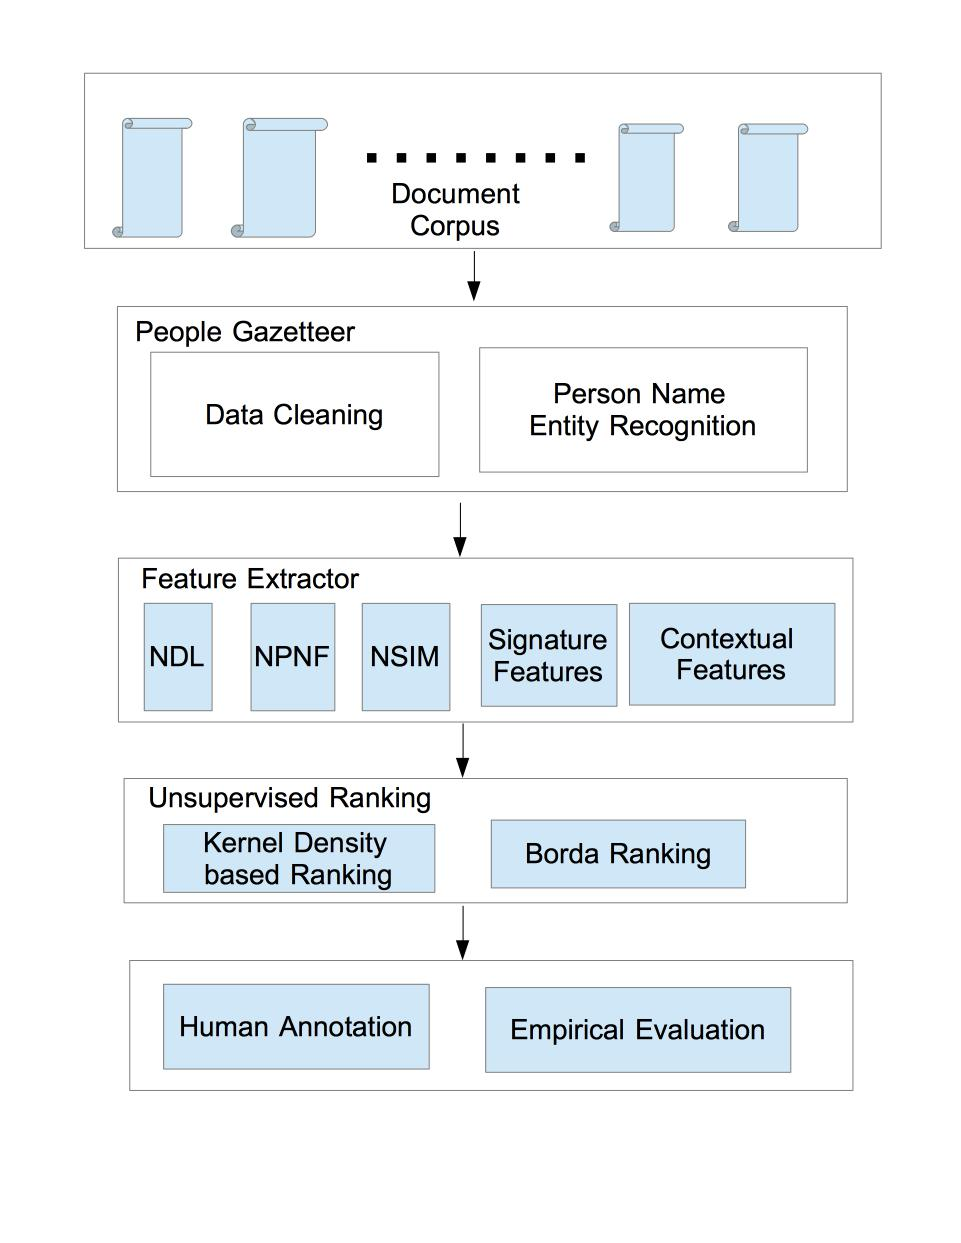
\includegraphics[width=0.38\textheight]{arch.jpg}
    \caption{Reputation System for Person Name Entities}
    \label{arch}
\end{center}   
\end{figure}


\subsection{Document Ingestion Layer}
%\begin{itemize}
%\item Document Ingestion Layer: 
This layer is responsible for maintaining the document corpus, including keeping track of the time window during which they are generated. Our system is shown to work with two document corpora -- a subset of articles obtained from the historical archive of ``The Sun" newspaper from Nov. 1894 and a more recent ``Washington Post" corpus. 

\subsection{People Gazetteer} It consists of tuples comprising of person names along with the list of documents in which they occur. To build the gazetteer, a Named Entity Recognizer (NER\footnote{The Stanford CRF-NER\footnote{http://nlp.stanford.edu/software/CRF-NER.shtml} (\cite{mccallum2003early, finkel2005incorporating, sutton2011introduction})  is used for Person Named Entity Recognition. }) is run on every document in the corpus to mark up people names occurring in the text. This process involves \emph{chunking} or segmentation of the text, followed by classification of the name by entity type (for e.g. person, organization, and location). Only multi-term entities of type ``person" are retained. Repetitions of entity names are not allowed -- for example, if the person names ``John", ``John Smith", ``Smith" are recognized, we only consider ``John Smith" as an entry for the gazetteer. For the historical newspaper archive, a total of 36364 person entities are extracted from 14020 news articles. [ENTRY DETAILS ABOUT WASHINGTON POST]
Once the gazetteer is built, features are extracted and reputed people need to be identified.

\subsection{Feature Extractor} We extract several features corresponding to each person in the gazetteer. These are:

\begin{enumerate}
\item \textbf{Normalized Document Length (NDL): } Document Length is defined as the number of tokens contained in a news article. It is further normalized by dividing with the maximum length of any news article across the corpus. Thus,  
$NDL= \frac{\text{Document Length}} {\text{Maximum Document Length in the dataset}}$

%\item[$\bullet$IDF]
%IDF is used as a parameter in the calculation of DI of a news article to give weight to the person entity's occurrence in the complete %dataset. It can be calculated as the number of news articles in which a person entity occurs in the complete dataset. It is %equivalent to the length of document list in the people gazetteer for each person entity.

%\item
\item \textbf{ Normalized Person Name Frequency (NPNF): }
Person Name Frequency (PNF) accounts for the number of occurrences of a person's name in the news article. A high value of PNF makes the document more important. It is normalized as follows:

\begin{center}
$NPNF=	1+\log$(PNF)
\end{center}

\item \textbf{Number of similar articles (NSIM): }
%This parameter is used in the calculation of the DI by finding articles belonging to the same topic. 
%The set of topics derived from a corpus can be used to answer questions about the similarity of words and 
%documents.
For a document $d$, let  SIM= Number of articles with the same topic as $d$ in the document list of a person.
This measure is normalized by the total number of articles in the document list of the person. Formally,

%\begin{center}
$NSIM= \frac{\text{SIM}} {\text{Total number of articles in the person's document list}}$
%\end{center}
NSIM is equivalent to the proportion of topic similar articles that document $d$ has.
%This parameter takes into account the effect of a document's score on a person's IPI when there exist several other documents of the same topic in the person's list. 
%\end{enumerate}

\item \textbf{Signature Features: } For every person name identified, we examine the words before it to identify occurrences of specific titles. Titles are assumed to signify veneration, official position and academic  or professional qualifications. We use this as an indicator of whether a person is reputed or not. Specifically, we use the categorization of titles from the Wikipedia\footnote{https://en.wikipedia.org/wiki/Title} page but only restrict it to the following categories: legislative and executive, aristocratic (both genders are considered), judicial, ecclesiastical, academic, military, and ranks of other organizations. For each category, we examine the occurrence of the title before the person name -- the feature value is set to 1 if it does occur and 0 otherwise.

\item \textbf{Contextual Features: } The entire text in the document is used to extract features. Word2Vec representation (\cite{Mikolov_13a, Mikolov_13b}) of the text is obtained using the deeplearning4j framework (\url{https://deeplearning4j.org/word2vec}) -- the input to the word2vec two layer neural net is the text in the document and the output is a 100 dimensional representation of words; these vectors, called \emph{neural word embeddings}, are obtained using a continuous bag of word representation (CBOW). 

\end{enumerate}
The above features are used in our unsupervised ranking models.


\subsection{Ranking Models }
The objective is to rank the set of all person names in the corpus based on reputation. Towards this end, a set of features denoted by $f_1,f_2, \cdots, f_n$ is extracted which provides the basis for ranking. Two different unsupervised ranking models are used in this work. These are described below:
\begin{enumerate}
\item \textbf{Kernel Density Estimation (KDE) based Ranking: } In this method, we assume that the most reputed person can be found by looking for peaks in a simple probabilistic model of the documents. The probability of a person being reputed is modeled as $P(P_j = reputed) = P(f_1,f_2 \cdots, f_n)$. We learn the probabilities of our model by estimating the non-parametric densities (\cite{scott_multivariate_2015, Silverman86}) of all features learnt from the corpus. Specifically, let $X \subseteq R^n$ be the domain of interest with $n$-features and $f: X \rightarrow R_{\ge 0}$ be an unknown probability density function. Let $D \subseteq X$ be a set of samples drawn from $f$. For any $x \in X$ we estimate $f(x)$ by using the function:
\begin{equation}
\label{eqn1}
\hat{f}_D(x) = \frac{1}{|D|} \sum_{s \in D} \prod_{i=1}^{n} \frac{1}{h_i} K(\frac{x_i - s_i}{h_i})
\end{equation}
where $x_i$ and $s_i$ are the $i^{th}$ components of $x$ and $s$ respectively and $h_i$ is the $i^{th}$ component of the bandwidth vector $h$. $K$ is the kernel function and the kernel function chosen in this work is the Gaussian kernel. The choice of the bandwidth vector $h$ is critical. Of the several known choices, the normal plug-in method is used here:
\begin{equation}
\label{eqn2}
h_i = (\frac{4}{|D| (n+2)})^{\frac{1}{n+4} \hat{\sigma_i}}
\end{equation}
where $ \hat{\sigma_i}$ is the sample standard deviation computed from the $i^{th}$ column of $|D|$.

Finally, the rank of a person based on reputation, is inversely proportional to the probability of being reputed computed using the KDE based ranking.  

 \item \textbf{Borda Ranking: } The Borda (\cite{Borda_81}) method is a rank aggregation scheme used commonly in literature (\cite{Dwork_01}). Given a set of rankings $f_1, f_2, \cdots, f_m$ of the set of person names $X_1, X_2, \cdots, X_n$, the objective is to produce a single ranking $R$ that is in agreement with the existing rankings. Borda's method first assigns a score $B_i(c)=$ the number of candidates ranked below $c$ in $f_i$ and then the total Borda score $B(c)$ is defined as $\sum_{i=1}^{m} B_i(c)$. Ties are resolved by averaging the rank over the person names having same score. Next, ranks across $f_1, f_2, \cdots, f_m$ are averaged to calculate the aggregated rank for each person. This average rank is sorted in descending order to obtain the final ranked list of person names.
 
\end{enumerate}

%\item {Human Annotation: }

\subsection{Evaluation of Models } We use the notion of a top-$K$ lists, ubiquitously used in the information retrieval community, for comparing ranked lists. Several metrics, such as precision and recall at various values of $K$, are used to assess the quality of the top-$K$ lists. These metrics, however, are computed by comparing them against a ``ground truth". The notion of ``ground truth" is hard to define in our application and even if it existed, it is likely to be very subjective. In addition, these metrics provide an absolute (unary) rating rather than a relative notion of distance. What is most relevant in our setting, therefore, is to be able to compare two top-$K$ lists for similarity/dissimilarity. We adapt two metrics (Spearman's footrule and Kendall Tau) for comparing top-$K$ lists proposed by Fagin et al. (\cite{Fagin_03}) and define them here for the sake of completeness.

A permutation $\sigma$ is a bijection from the set $D = D_{\sigma}$ (also called domain or universe) onto a set $[n] = \{1,2, \cdots, n\}$ where $[n]$ is the size of $|D|$. Let $S_{D}$ be the set of all permutations of $D$. For a given permutation $\sigma$, $\sigma(i)$ refers to the rank of element $i, i \le i \le n$. If $\sigma(i) < sigma(j)$, then $i$ is ranked ahead of $j$. Let $\mathcal{P}=\mathcal{P}_D = \{(i,j) | i, j \in D\}$ be the set of unordered pairs of objects in $D$ and $\sigma_1, \sigma_2 \in S_D$. 

\noindent \textbf{Kendall Tau ($KT(\sigma_1, \sigma_2)$):} For each pair $(i,j) \in \mathcal{P}$, if $i, j$ are in the same order in $\sigma_1, \sigma_2$, then $K_{i,j} (\sigma_1, \sigma_2)=0$, else if $i, j$ are in reverse order i.e. $i$ is before $j$ in $\sigma_1$, but $j$ is before $i$ in $\sigma_2$, then $K_{i,j} (\sigma_1, \sigma_2)=1$. Thus, Kendall Tau = $KT(\sigma_1, \sigma_2)=\sum_{{i,j} \in \mathcal{P}} K_{i,j} (\sigma_1, \sigma_2)$.

\noindent \textbf{Spearman's Footrule ($F(\sigma_1, \sigma_2)$): } This is given by the $L_1$ distance between two permutations i.e. $F(\sigma_1, \sigma_2) = \sum_{i=1}^n |\sigma_1(i) - \sigma_2(i)|$.

The above two metrics traditionally used for comparing ranked lists are further adapted to work with top-$K$ lists. Given two top-$K$ lists $\tau_1$ and  $\tau_2$, we define $\mathcal{P}(\tau_1, \tau_2) = \mathcal{P}_{D_1 \cup D_2}$ to be the set of all unordered pairs of elements in $D_{\tau_1} \cup D_{\tau_2}$. For top-$K$ lists, the minimizing Kendall Tau metric between two top-$K$ lists $KT_{min}(\tau_1, \tau_2)= \text{min} K_{i,j} (\sigma_1, \sigma_2)$ where $\sigma_1, \sigma_2$ are permutations of $D_{\tau_1} \cup D_{\tau_2}$ and where $\sigma_1 \succeq \tau_1$ and $\sigma_2 \succeq \tau_2$.

To estimate the Spearman's Footrule for top-$K$ lists ($F^{l}(\tau_1, \tau_2)$), we observe that there exists a real number $l$ greater than $K$. The Footrule with location parameter $l$ is obtained by placing all the missing elements in each of the lists at position $l$ and then estimating Footrule in the usual manner. Thus given top-$K$ lists, $\tau_1$ and $\tau_2$ we define $\hat{\tau_1}$ and  $\hat{\tau_2}$ with domain  $D_{\tau_1} \cup D_{\tau_2}$ i.e. $\hat{\tau_1} = \tau_i, \text{for } i \in D_{\tau_1} \text{and } \hat{\tau_1} = l$, otherwise. $\hat{\tau_2}$ is similarly defined. Then, $F^{l}(\tau_1, \tau_2)= \sum_{i \in D_{\tau_1} \cup D_{\tau_2}} | \hat{\tau_1} - \hat{\tau_2}|$.
% \end{itemize} 

\section{Data Description}
\label{data}
Two data sets are used to provide empirical validation of the claim that unsupervised ranking schemes can be used for finding reputed people. These are as follows:

\begin{enumerate}
\item Historical Newspaper Archive: Historical newspapers are obtained from Chronicling America\footnote{\texttt{http://chroniclingamerica.loc.gov/}}. Under this program, institutions such as libraries receive an award to select and digitize approximately 100,000 newspaper pages representing that state's regional history, geographic coverage, and events of the particular time period being covered. The scanned newspaper holdings of the New York Public Library are a source of prosopographical studies. The newspapers are scanned on a page-by-page basis and article level
segmentation is poor or non-existent; the OCR scanning process is far
from perfect and the documents generated from it contain a large
amount of garbled text. Article level segmentation of text is available for only two months -- since this requires human intervention. Articles of ``The Sun" newspaper from November-December 1894 consisting of 14020 news articles are used in our study. 

\textbf{Pre-processing: } The garbled OCR text makes data preprocessing mandatory before application of any text mining algorithms. We,therefore, use edit distance algorithm based on Levenshtein distance to perform spelling correction on the OCR text articles. The algorithm is chosen because of its speed and ability to correct OCR errors compared to the n-gram approach \cite{chattopadhyaya2013fast}. Our edit distance algorithm also uses an enhanced person names dictionary for look up to give significance to personal names spelling correction in the dataset. The results of spelling correction and data preprocessing are presented in \cite{Gupta_14a}.


\item Contemporary Newspaper Archive: [DESCRIBE THE WASHINGTON POST DATA]
\end{enumerate}

%\subsection{Pre-processing}



\section{Empirical Results}
\label{emp}

\subsection{Aims}
The objective of the empirical study reported in this section is to test the effectiveness of using the unsupervised ranking algorithm based on Kernel Density Estimation in the reputation management system for person name entities. Towards this end, we would like to answer the following questions: (a) How does the proposed unsupervised ranking algorithm based on Kernel Density Estimation compare to rank aggregation schemes known in literature (for e.g. Borda score)? (b) What is the effect of varying parameters (for e.g. the number of points at which the density is estimated, the method of bandwidth selection) of the KDE algorithm on the top-$K$ ranked list?  

\subsection{Results}
\textbf{Comparison of KDE based ranking algorithm to Borda rank aggregation scheme:}
The performance of the unsupervised ranking algorithm is presented on both the data sets described in Section~\ref{data}. Figure~\ref{KDEBorda-OCR} compares the performance of the Kernel Density Estimation technique with a rank aggregation scheme, Borda ranking on the Historical Newspaper Archive data. In both the cases the top-50 elements of the ranked lists are examined and the Kendall-Tau and Spearman's Footrule distance between them are reported. For the KDE technique, the number of data points at which the density is estimated is varied to be 50, 100, 250, 500 and 1000. The top-50 lists (KDE and Borda) are most similar when the Kernel Density is estimated at 100 sample points as reflected in both the Kendall-Tau and Spearman's Footrule measures.

\begin{figure}[H]
\begin{center}
   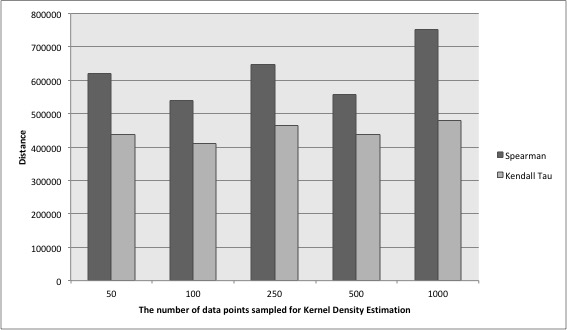
\includegraphics[width=0.38\textheight]{KDEBorda.jpg}
    \caption{Comparison of the unsupervised ranking algorithm based on Kernel Density Estimation to Borda rank aggregation scheme on the Historical Newspaper Archive data. The top-50 elements of the ranked list are compared using both the schemes. The x-axis plots the number of data points at which the density is estimated for the KDE based ranking scheme. The y-axis reports the Kendall-Tau or Spearman's Footrule distance between the ranked lists. }
    \label{KDEBorda-OCR}
\end{center}   
\end{figure}

\textbf{Study of the effect of varying parameters of the kernel density estimation scheme on ranking results:}

\begin{figure}[H]
\begin{center}
   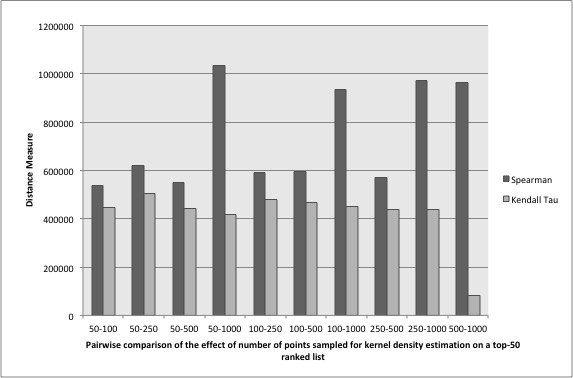
\includegraphics[width=0.38\textheight]{VaryingNoOfPtsKDE.jpg}
    \caption{The effect of varying the number of points at which the density is estimated on the Historical Newspaper Archive dataset.}
    \label{KDEVaryNoOfPts}
\end{center}   
\end{figure}


Several parameters of the Kernel Density Estimation scheme are varied to test the effect on ranking performance. These are: (a) The number of points at which the density is estimated: Figure~\ref{KDEVaryNoOfPts} presents the results on the Historical Newspaper Archive data. Our results indicate that the ranked lists obtained when 50 and 100 data points are sampled are quite similar to one another. However, the lists are significantly different when 1000 or more points are sampled. 


\subsection{Discussions}

\section{Related Work}
\label{related}
\subsection{Extraction of reputed people names from text documents}

%% Jayashree please write this section

\subsection{Ranking of named entities}

%% Aayushee Please Update This Section
- Discuss supervised and unsupervised ranking methods \\
- Talk about Rank Aggregation schemes \\



\section{Conclusion}
\label{conc}

This paper presents a reputation system for person named entities using an unsupervised ranking scheme based on kernel density estimation. Person names are extracted from newspaper articles and are added to a people gazetteer. Several textual features that are likely to affect the reputation of a person such as the context in which s/he was discussed, the length of the articles, other similar articles in which they are discussed, and titles by which s/he was addressed are extracted. These features are used by an unsupervised kernel density based ranking algorithm to generate a top-$K$ list. The parameters of the kernel density based ranking algorithm are compared to other state-of-the-art rank aggregation schemes such as Borda aggregation. Furthermore, human annotators test the quality of our top-$k$ ranked list and verify that our system is able to learn the reputation of people names extracted from the archives. Our results on two data sets -- one historical and another a contemporary newspaper archive -- indicate that the kernel density based ranking algorithm is useful in designing reputation systems.

\section{Acknowledgements}
The authors would like to thank Arpit Rana for help with annotations.
%\subsection{Comments}
%
%You can add inline TODO comments with the todonotes package, like this:
%\todo[inline, color=green!40]{This is an inline comment.}
%
%\subsection{References}
%
%LaTeX automatically generates a bibliography in the APA style from your .bib file. The citep command generates a formatted citation in parentheses \citep{Lamport1986}. The cite command generates one without parentheses. LaTeX was first discovered by \cite{Lamport1986}.



% Commands to include a figure:
%\begin{figure}
%\centering
%\includegraphics[width=0.5\textwidth]{frog.jpg}
%\caption{\label{fig:frog}This is a figure caption.}
%\end{figure}


\bibliography{jasist}
%\printbibliography

\end{document}

%
% Please see the package documentation for more information
% on the APA6 document class:
%
% http://www.ctan.org/pkg/apa6
%